%versi 2 (8-10-2016)
\chapter{Landasan Teori}
\label{chap:teori}

\section{Linear Programming}
\label{linear_programming}

Linear programming adalah teknik dalam ilmu matematika untuk menyelesaikan masalah yang berhubungan dengan optimasi. Teknik ini biasa digunakan dalam bidang produksi, manajemen operasional, penjadwalan, dan bidang-bidang lainnya yang melibatkan pengambilan keputusan. Pada bidang produksi, terdapat masalah ketika menentukan produk yang akan dihasilkan. Biasanya terdapat beberapa faktor yang menjadi pertimbangan seperti jumlah ketersedian sumber daya, jumlah pekerja, dan besar keuntungan yang didapatkan. Dengan adanya faktor-faktor tersebut, penentuan terhadap produk yang akan dihasilkan tentunya harus dilakukan dengan perhitungan yang tepat. Linear programming merupakan teknik yang cocok untuk menyelesaikan masalah tersebut. Dengan memodelkan masalah tersebut secara tepat, maka masalah tersebut dapat diselesaikan sehingga menghasilkan solusi terbaik tanpa mengabaikan setiap faktor yang ada.

\subsection{Karakteristik}
\label{karakteristik}

Setiap masalah optimasi dapat dimodelkan ke dalam bentuk masalah linear programming. Masalah linear programming memiliki ciri-ciri sebagai berikut:

\begin{itemize}
	\item Variabel keputusan
	
		Di dalam masalah linear programming terdapat variabel-variabel keputusan. Variabel keputusan menunjukkan keputusan yang diambil.
		
		\begin{equation*}
			\begin{split}
				x_1 &= \text{jumlah produk A yang diproduksi} \\
    			x_2 &= \text{jumlah produk B yang diproduksi}
			\end{split}
		\end{equation*}
		
	\item Fungsi Tujuan
	
		Di dalam masalah linear programming terdapat tujuan yang akan dicapai. Tujuan ini dimodelkan dengan memaksimalkan/meminimalkan variabel-variabel keputusan.
		
		\begin{equation*}
			\text{maximize } z = 3x_1 + 2x_2
		\end{equation*}

	\item Batasan
	
		Batasan dalam linear programming berfungsi untuk membatasi nilai variabel. Batasan juga dapat menunjukkan keterkaitan antar variabel keputusan.
		%Fungsi tujuan ditentukan oleh variabel-variabel keputusan. Dalam fungsi tujuan yang memaksimalkan hasil, nilai dari setiap variabel keputusan dapat ditentukan sedemikian mungkin sehingga menghasilkan hasil sebesar-besarnya. Tentunya hal ini tidak mungkin terjadi karena terdapat faktor-faktor yang mencegah variabel keputusan untuk ditentukan sedemikian mungkin. Faktor-faktor ini berperan sebagai batasan bagi variabel keputusan sehingga nilai variabel keputusan tidak melebihi batas. Dengan adanya batasan ini, nilai dari fungsi tujuan tidak akan bernilai tak hingga karena variabel-variabel keputusannya dibatasi.
		
		\begin{equation*}
			\begin{split}
				2x_1 + x_2 &\leq 100 \\
    			x_1 + x_2 &\leq 80 \\
    			x_1 &\leq 40
			\end{split}
		\end{equation*}
		
	\item Tanda Pembatas
		
		Tanda pembatas berfungsi untuk menyatakan apakah variabel keputusan dapat bernilai negatif atau tidak. Jika variabel keputusan \(x_i\) tidak dapat bernilai negatif maka perlu ditambahkan tanda pembatas \(x_i \geq 0\). Namun, apabila nilai variabel keputusan tidak dibatasi atau dapat bernilai negatif, maka variabel keputusan tersebut merupakan variabel bebas (\textit{unrestricted in sign}).
		
		\begin{equation*}
			\begin{split}
    			x_1 &\geq 0 \\
    			x_2 &\geq 0
			\end{split}
		\end{equation*}
		
\end{itemize}

Dengan keempat karakteristik di atas, setiap masalah optimasi dapat dimodelkan ke bentuk masalah linear programming. Berikut contoh masalah linear progamming:

\begin{equation*}
	\begin{array}{r r c r c l}
		\text{maximize} &\multicolumn{5}{l}{z = 3x_1 + 2x_2}\\
		\text{subject to} &2x_1 &+ &x_2 &\leq &100\\
		&x_1 &+ &x_2 &\leq &80\\
		&x_1 &&&\leq &40\\
		&x_1 &&&\geq &0\\
		&&&x_2 &\geq &0\\
	\end{array}
\end{equation*}

\subsection{Daerah Solusi dan Solusi Optimal}
\label{daerah_solusi_dan_solusi_optimal}

Di dalam linear programming terdapat daerah solusi. Setiap batasan pada masalah linear programming akan menentukan daerah yang memenuhi batasan tersebut. Irisan dari gabungan daerah-daerah tersebut akan menghasilkan daerah solusi bagi masalah linear programming. Dengan adanya daerah solusi, maka masalah linear programming dapat diselesaikan karena memiliki solusi yang dibatasi.

%Solusi dari linear programming merupakan solusi yang tidak melanggar setiap batasan-batasannya. Dengan diketahuinya hal ini, bisa saja maka linear programming memiliki banyak solusi dengan tidak melanggar batasan manapun. Dalam linear programming, solusi-solusi ini berada dalam daerah yang disebut dengan daerah solusi (feasible reqion). Daerah ini berbentuk \textit{covex polytope} yang terdiri dari banyak titik sudut. Titik-titik sudut ini merupakan perpotongan dari setiap batasan dengan batasan-batasan lainnya. Dengan adanya daerah ini, pencarian solusi menjadi dibatasi sehingga tidak perlu memeriksa seluruh kemungkinan yang ada. 

%Bila diketahui bahwa titik sudut dibentuk dari perpotongan antar batasan, maka hal ini tidak berlaku sebaliknya. Titik potong tidak selalu menjadi titik sudut bagi daerah solusi. Titik sudut merupakan titik potong yang tidak melanggar batasan-batasan. Apabila daerah solusi divisualisasikan dalam bentuk grafik atau lainnya, daerah solusi akan berbentuk \textit{convex polytope}.

%Bila daerah solusi sudah ditemukan, solusi optimal dapat dicari dengan memeriksa setiap kemungkinan yang berada di dalam daerah solusi. Walaupun demikian, pemeriksaan ini masih dianggap tidak efisien. Bila solusi optimal dapat berupa bilangan pecahan, maka pemeriksaan tidak dapat berakhir karena bilangan pecahan yang berada di antara dua batas berjumlah tak hingga.

%Tentunya seluruh pemeriksaan ini dapat dihindari karena solusi optimal dari linear programming berada pada salah satu titik sudut di daerah solusi. Dengan diketahuinya hal ini, maka solusi optimal dapat dicari dengan mengecek setiap titik sudut yang berjumlah terhitung (\textit{finite}).

Apabila memiliki daerah solusi, maka masalah linear programming tersebut memiliki solusi optimal. Daerah ini berbentuk \textit{convex polytope} yang terdiri dari banyak titik sudut. Solusi optimal bagi masalah linear programming terdapat pada salah satu titik sudut.

\begin{figure}[H]
	\centering
	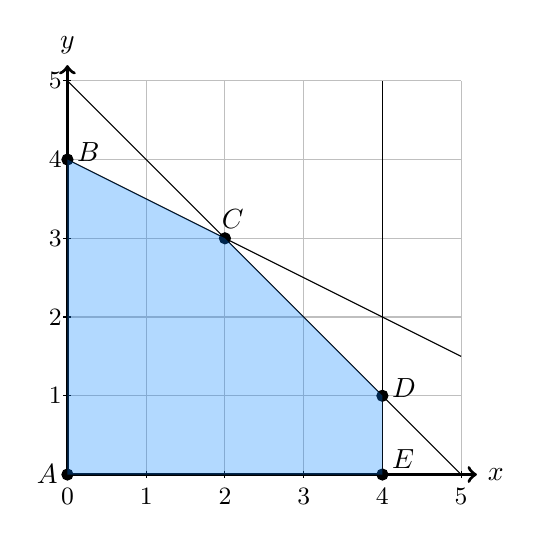
\begin{tikzpicture}
		\draw[gray!50, thin, step=1] (0,0) grid (5,5);
		\draw[very thick,->] (0,0) -- (5.2, 0) node[right] {$x$};
		\draw[very thick,->] (0,0) -- (0, 5.2) node[above] {$y$};
		\foreach \x in {0,...,5} \draw (\x,0.05) -- (\x,-0.05) node[below] {\small\x};
		\foreach \y in {1,...,5} \draw (-0.05,\y) -- (0.05,\y) node[left] {\small\y};
		\draw (0,4) -- (5, 1.5);
		\draw (4,0) -- (4,5);
		\draw (0,5) -- (5,0);
		\filldraw [black] (0,0) circle (2pt);
		\filldraw [black] (0,4) circle (2pt);
		\filldraw [black] (2,3) circle (2pt);
		\filldraw [black] (4,1) circle (2pt);
		\filldraw [black] (4,0) circle (2pt);
		\draw (0,0) node[left] {$A$};
		\draw (0,4.1) node[above,right] {$B$};
		\draw (2.1,3) node[above] {$C$};
		\draw (4,1.1) node[right] {$D$};
		\draw (4,0.2) node[right] {$E$};
		\fill[blue!50!cyan,opacity=0.3] (0,0) -- (0,4) -- (2,3) -- (4,1) -- (4,0) -- cycle;
	\end{tikzpicture}
	\caption{Daerah solusi dan titik-titik sudut}
\end{figure}

Terdapat 3 jenis daerah solusi dalam masalah linear programming, yaitu:

\begin{enumerate}
	\item Daerah solusi yang dibatasi (\textit{bounded feasible region})
	
		Batasan-batasan menghasilkan daerah solusi yang berbentuk \textit{convex polytope}. Solusi optimal linear programming terdapat pada salah satu titik sudut.
			
		\begin{figure}[H]
    		\centering
			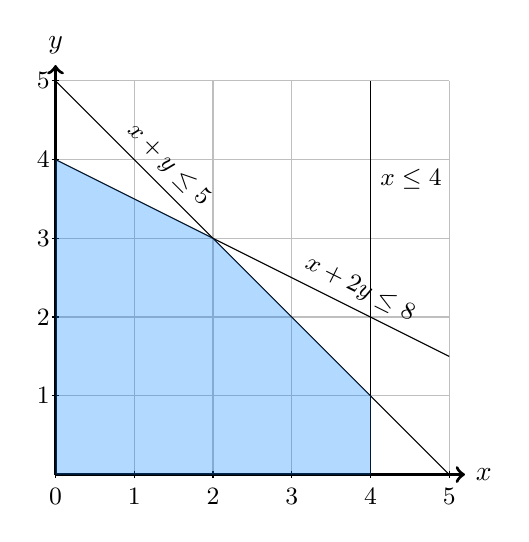
\begin{tikzpicture}
		    	\draw[gray!50, thin, step=1] (0,0) grid (5,5);
				\draw[very thick,->] (0,0) -- (5.2, 0) node[right] {$x$};
				\draw[very thick,->] (0,0) -- (0, 5.2) node[above] {$y$};
				\foreach \x in {0,...,5} \draw (\x,0.05) -- (\x,-0.05) node[below] {\small\x};
				\foreach \y in {1,...,5} \draw (-0.05,\y) -- (0.05,\y) node[left] {\small\y};
				\draw (0,4) -- node[above,near end,sloped] {\small $x + 2y \leq 8$} (5, 1.5);
				\draw (4,0) -- node[right,near end] {\small $x \leq 4$} (4,5);
				\draw (0,5) -- node[above,near start,sloped] {\small $x + y \leq 5$} (5,0);
				\fill[blue!50!cyan,opacity=0.3] (0,0) -- (0,4) -- (2,3) -- (4,1) -- (4,0) -- cycle;
			\end{tikzpicture}
			\caption{Daerah solusi yang dibatasi}
		\end{figure}
    	
	\item Daerah solusi yang tidak dibatasi (\textit{unbounded feasible region})
	
		Batasan-batasan menghasilkan daerah solusi yang tidak tertutup sehingga tidak berbentuk \textit{convex polytope}. Daerah solusi ini memiliki jumlah solusi yang tak terhitung.
			
    	\begin{figure}[H]
    		\centering
			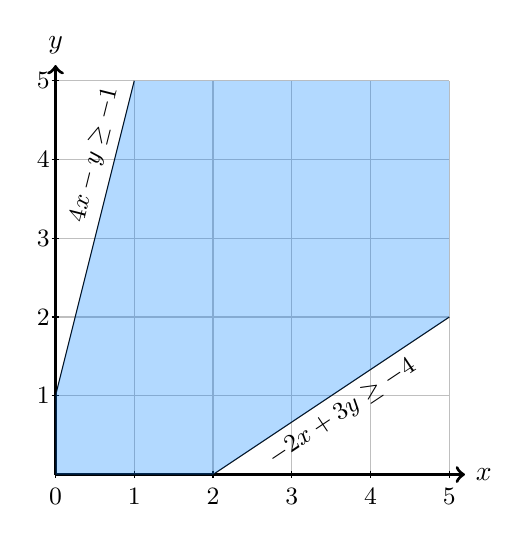
\begin{tikzpicture}
				\draw[gray!50, thin, step=1] (0,0) grid (5,5);
				\draw[very thick,->] (0,0) -- (5.2, 0) node[right] {$x$};
				\draw[very thick,->] (0,0) -- (0, 5.2) node[above] {$y$};
				\foreach \x in {0,...,5} \draw (\x,0.05) -- (\x,-0.05) node[below] {\small\x};
				\foreach \y in {1,...,5} \draw (-0.05,\y) -- (0.05,\y) node[left] {\small\y};
				\draw (2,0) -- node[below,sloped] {\small $-2x + 3y \geq -4$} (5,2);
				\draw (0,1) -- node[above,near end,sloped] {\small $4x - y \geq -1$} (1,5);
				\fill[blue!50!cyan,opacity=0.3] (0,0) -- (0,1) -- (1,5) -- (5,5) -- (5,2) -- (2,0) -- cycle;
			\end{tikzpicture}
			\caption{Daerah solusi yang tidak dibatasi}
		\end{figure}

	\item Tidak ada daerah solusi (\textit{infeasible region})

		Batasan-batasan tidak membentuk daerah solusi sehingga masalah linear programming tidak memiliki solusi dan tidak dapat diselesaikan.
			
		\begin{figure}[H]
    		\centering
			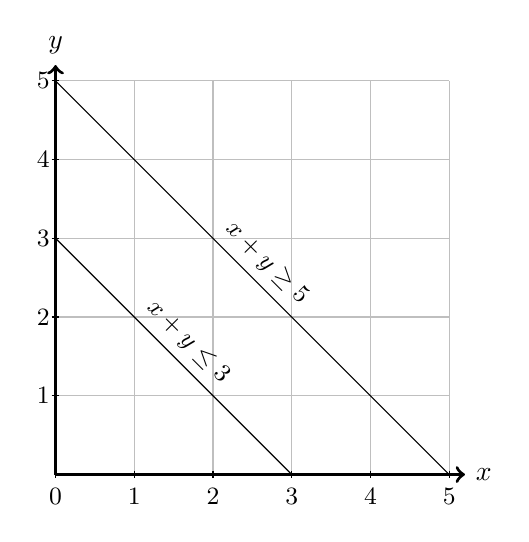
\begin{tikzpicture}
				\draw[gray!50, thin, step=1] (0,0) grid (5,5);
				\draw[very thick,->] (0,0) -- (5.2, 0) node[right] {$x$};
				\draw[very thick,->] (0,0) -- (0, 5.2) node[above] {$y$};
				\foreach \x in {0,...,5} \draw (\x,0.05) -- (\x,-0.05) node[below] {\small\x};
				\foreach \y in {1,...,5} \draw (-0.05,\y) -- (0.05,\y) node[left] {\small\y};
				\draw (3,0) -- node[above,sloped] {\small $x + y \leq 3$} (0,3);
				\draw (5,0) -- node[above,sloped] {\small $x + y \geq 5$} (0,5);
			\end{tikzpicture}
			\caption{Tidak ada daerah solusi}
    	\end{figure}

\end{enumerate}

\subsection{Bentuk Standar}
\label{bentuk_standar}

Setiap model linear programming dapat dimodelkan ke dalam bentuk standar seperti berikut ini:
    	
\begin{equation*}
	\begin{array}{r r c r c r c r c l}
	    \text{maximize}		& c_1x_1    & + & c_2x_2 	& + & \dots & + & c_nx_n \\
		\text{subject to} 	& a_{11}x_1 & + & a_{12}x_2 & + & \dots & + & a_{1n}x_n & = & b_1 \\
    						& a_{21}x_1 & + & a_{22}x_2 & + & \dots & + & a_{2n}x_n & = & b_2 \\
                            & \multicolumn{7}{c}{\vdots}                            &   & \vdots \\
                            & a_{m1}x_1 & + & a_{m2}x_2 & + & \dots & + & a_{mn}x_n & = & b_m \\
                            & \multicolumn{9}{l}{x_1\geq0,x_2\geq0,\dots,x_n\geq0}
	\end{array}
\end{equation*}

Bentuk tersebut merupakan bentuk standar masalah linear programming yang terdiri dari $n$ buah variabel $x$ dan $m$ buah persamaan batasan. Variabel $b_i,c_i,a_{ij}$ merupakan konstanta dan $x_i$ merupakan variabel keputusan. 

Bentuk standar tersebut dapat dinyatakan dalam notasi matriks seperti berikut ini:
        
\begin{center}
	\begin{tabular}{r l}
    	\textit{maximize}   & $c^Tx$ \\
        \textit{subject to} & $Ax=b$ and $x\geq0$
	\end{tabular}    
\end{center}
        
Pada notasi matriks, $x$ adalah matriks kolom berdimensi $n$, $C^T$ adalah matriks baris berdimensi $n$, $A$ adalah matriks berdimensi $m\times n$, dan $b$ adalah matriks kolom berdimensi $m$. Matriks $x\geq0$ menunjukkan variabel keputusan $x_i$ tidak dapat bernilai negatif.
        
Langkah-langkah untuk mengubah masalah linear programming ke bentuk standar:

\begin{enumerate}
%	\item Ubah tujuan agar memaksimalkan
	
%		Apabila bertujuan meminimalkan, maka ubah tujuan agar memaksimalkan dengan cara mengalikan fungsi tujuan dengan -1. Contoh:

%		\begin{equation*}
%			\text{minimize } z = x_1 + 2x_2
%		\end{equation*}
		
%		menjadi
		
%		\begin{equation*}
%			\text{maximize } -z = -x_1 - 2x_2
%		\end{equation*}
		
%	\item Ubah sisi kanan pertidaksamaan batasan sehingga tidak bernilai negatif
	
%		Apabila konstanta di sisi kanan pada pertidaksamaan batasan berupa bilangan negatif, maka kalikan kedua ruas pertidaksamaan dengan -1 sehingga sisi kanan tidak bernilai negatif. Contoh:
		
%		\begin{equation*}
%			x_1 + 2x_2 \leq -20
%		\end{equation*}
		
%		menjadi
		
%		\begin{equation*}
%			-x_1 - 2x_2 \geq 20
%		\end{equation*}

	\item Mengubah batasan ke dalam bentuk persamaan
	
		Perubahan pertidaksamaan pada batasan dibedakan menjadi 2 berdasarkan jenis tandanya, yaitu:
		
		\begin{enumerate}
			\item Pertidaksamaan lebih kecil (\(\leq\))		

				Pertidaksamaan dengan tanda lebih kecil diubah ke bentuk persamaan dengan menambahkan variabel baru positif bernama \textit{slack}. Lalu tambahkan tanda pembatas tidak negatif untuk variabel \textit{slack} tersebut. Contoh:
				
				\begin{equation*}
					x_1 + 2x_2 \leq 40
				\end{equation*}
				
				menjadi
				
				\begin{equation*}
					\begin{split}
						x_1 + 2x_2 + s_1 &= 40\\
						s_1 &\geq 0
					\end{split}
				\end{equation*}
			
			\item Pertidaksamaan lebih besar (\(\geq\))
			
				Pertidaksamaan dengan tanda lebih besar diubah ke bentuk persamaan dengan menambahkan variabel baru negatif bernama \textit{surplus}. Lalu tambahkan tanda pembatas tidak negatif untuk variabel \textit{surplus} tersebut. Contoh:
				
				\begin{equation*}
					x_1 + 2x_2 \geq 40
				\end{equation*}
				
				menjadi
				
				\begin{equation*}
					\begin{split}
						x_1 + 2x_2 - e_1 &= 40\\
						e_1 &\geq 0
					\end{split}
				\end{equation*}
		\end{enumerate}
		
	\item Mengsubtitusi variabel bebas
	
		Apabila terdapat variabel bebas \(x_i\), maka subtitusikan setiap variabel tersebut dengan 2 variabel pengganti \(u_i\) dan \(v_i\) sehingga \(x_i = u_i - v_i\). Lalu tambahkan tanda pembatas tidak negatif untuk variabel \(u_i\) dan \(v_i\). Contoh:
		
		\begin{equation*}
			\begin{array}{r r c r c l}
				\text{maximize} & \multicolumn{5}{l}{z = x_1 + x_2}\\
				\text{subject to} & 2x_1 & + & x_2 & \leq & 4\\
									& \multicolumn{3}{r}{x_1} & \geq & 0\\
			\end{array}
		\end{equation*}
		
		dengan
		
		\begin{equation*}
			x_2 = u_2 - v_2
		\end{equation*}
		
		menjadi
		
		\begin{equation*}
			\begin{array}{r r c r c r c l}
				\text{maximize} & \multicolumn{7}{l}{z = x_1 + u_2 - v_2}\\
				\text{subject to} & 2x_1 & + & u_2 & - & v_2 & \leq & 4\\
									& \multicolumn{5}{r}{x_1} & \geq & 0\\
									& \multicolumn{5}{r}{u_2} & \geq & 0\\
									& \multicolumn{5}{r}{v_2} & \geq & 0\\
			\end{array}
		\end{equation*}
\end{enumerate}

\subsection{Variabel Basis dan Non Basis}
\label{variabel_basis_dan_non_basis}

Masalah linear programming \(Ax = b\) yang terdiri dari \(m\) buah persamaan batasan dan \(n\) buah variabel keputusan. Masalah linear programming \(Ax = b\) memiliki solusi basis yang didapatkan dengan membuat \(n - m\) buah variabel bernilai 0 dan menyelesaikan \(m\) buah variabel lainnya. Sebanyak \(n - m\) buah variabel yang dibuat bernilai 0 disebut variabel non basis. Sedangkan sebanyak \(m\) buah variabel lainnya disebut variabel basis. Variabel basis merupakan variabel yang diselesaikan setelah membuat variabel lain menjadi variabel non basis. Berikut contoh sistem persamaan linear:

\begin{equation*}
	\setlength\arraycolsep{1.5pt}
	\begin{array}{r c r c r c l}
		x_1 &+ &x_2 &  &    &= &3\\
		    &  &x_2 &+ &x_3 &= &-1
	\end{array}
\end{equation*}

Pada sistem persamaan linear di atas, dipilih sebanyak 3 - 2 = 1 (3 variabel dan 2 persamaan) buah variabel yang akan menjadi variabel non basis. Jika himpunan variabel non basis NBV = \(\{x_3\}\), maka himpunan variabel basis BV = \(\{x_1, x_2\}\). Solusi dari sistem persamaan tersebut dapat dicari dengan membuat variabel \(x_3\) menjadi variabel non basis dan menyelesaikan variabel basis lainnya.

\begin{equation*}
	\begin{split}
		x_1 + x_2 &= 3\\
		-x_2 &= -1
	\end{split}
\end{equation*}

Pada persamaan di atas didapatkan nilai \(x_1\) = 2 dan \(x_2\) = 1. Dengan demikian didapatkan solusi basis \(x_1\) = 2, \(x_2\) = 1, \(x_3\) = 0.

\subsection{Metode Simplex}
\label{metode_simplex}

Metode simplex merupakan metode yang digunakan untuk mencari solusi optimal dari masalah linear programming. Metode simplex bekerja secara beriterasi dengan menghasilkan solusi yang mendekati optimal pada setiap iterasinya. Iterasi ini akan dilakukan hingga tidak ditemukannya solusi yang lebih optimal. Berikut contoh masalah linear programming:

\begin{equation*}
	\begin{array}{r c c c c l}
		\text{maximize}   & 3x_1 & + & 2x_2 \\
		\text{subject to} & 2x_1 & + & x_2  & \leq & 18 \\
        					& 2x_1 & + & 3x_2 & \leq & 42 \\
                           	& 3x_1 & + & x_2  & \leq & 24 \\
                           	& \multicolumn{5}{l}{x_1\geq0,x_2\geq0} \\
	\end{array}
\end{equation*}
        
Langkah-langkah untuk menyelesaikan maslaah linear programming dengan menggunakan metode simplex:

\begin{enumerate}
	\item Mengubah masalah ke dalam bentuk standar
	
        Masalah linear programming diubah ke bentuk standar sesuai dengan langkah-langkah yang sudah dibahas sebelumnya.
        
        Berikut contoh masalah linear programming yang sudah diubah ke bentuk standar:
        
	    \begin{equation*}
			\begin{array}{r c c c c c c c c c c l}
    	    	\text{maximize}   & 3x_1 & + & 2x_2 & + & 0x_3 & + & 0x_4 & + & 0x_5\\
	            \text{subject to} & 2x_1 & + & x_2  & + & x_3 &   &       &   &       & = & 18 \\
                        	   		& 2x_1 & + & 3x_2 &   &       & + & x_4 &   &       & = & 42 \\
                    	       		& 3x_1 & + & x_2  &   &       &   &       & + & x_5 & = & 24 \\
                	           		& \multicolumn{11}{l}{x_1\geq0,x_2\geq0,x_3\geq0,x_4\geq0,x_5\geq0} \\
        	\end{array}
		\end{equation*}
			
	\item Membuat tabel \textit{simplex}\\
		Tabel~\ref{tab:kerangka_tabel_simplex} merupakan kerangka tabel simplex yang terdiri dari 4 kolom utama, yaitu kolom basis, kolom $z$, kolom variabel non basis, dan kolom ruas kanan/rhs (\textit{right hand side}). Pada awalnya, baris $z$ berisi nilai negatif dari konstanta variabel pada fungsi tujuan dan $m$ baris berikutnya berisi konstanta variabel pada setiap persamaan batasan. $m$ baris terkahir ini diidentifikasikan sebagai baris basis.
        	
		\begin{table}[H]
			\centering
			\caption{Kerangka tabel simplex}
			\label{tab:kerangka_tabel_simplex}
			\begin{tabular}{|c|c|c c c c |c|}
				\hline
				basic & $z$ & $x_1$ & $x_2$ & \dots & $x_n$ & rhs \\
				\hline
				$z$ & 1 & $-c_1$ & $-c_2$ & \dots & $-c_n$ & 0 \\
				\hline
				$x_{n+1}$ & 0 & $a_{11}$ & $a_{12}$ & \dots & $a_{1n}$ & $b_1$ \\
				$x_{n+2}$ & 0 & $a_{21}$ & $a_{22}$ & \dots & $a_{2n}$ & $b_2$ \\
				\vdots & \vdots & \vdots & \vdots & \vdots & \vdots & \vdots \\
				$x_{n+m}$ & 0 & $a_{m1}$ & $a_{m2}$ & \dots & $a_{mn}$ & $b_m$ \\
				\hline
			\end{tabular}
		\end{table}
			
		Tabel~\ref{tab:contoh_simplex_awal} berikut adalah tabel simplex awal untuk contoh masalah linear programming.
			
		\begin{table}[H]
			\centering
			\caption{Tabel simplex awal}
			\label{tab:contoh_simplex_awal}
			\begin{tabular}{|c|c|c c c c c|c|}
				\hline
				basic & $z$ & $x_1$ & $x_2$ & $x_3$ & $x_4$ & $x_5$ & rhs \\
				\hline
				$z$ & 1 & -3 & -2 & 0 & 0 & 0 & 0 \\
				\hline
				$x_3$ & 0 & 2 & 1 & 1 & 0 & 0 & 18\\
				$x_4$ & 0 & 2 & 3 & 0 & 1 & 0 & 42\\
				$x_5$ & 0 & 3 & 1 & 0 & 0 & 1 & 24\\
				\hline
			\end{tabular}
		\end{table}

	\item Mengecek solusi optimal
	
    	Apabila pada baris $z$ tidak terdapat variabel dengan nilai negatif, maka solusi optimal sudah ditemukan dan menandakan akhir dari iterasi. Solusi optimal terdapat pada setiap rhs dari setiap baris basis. Jika masih terdapat variabel dengan nilai negatif, maka langkah selanjutnya adalah melakukan proses \textit{pivoting}.

		Pada Tabel~\ref{tab:contoh_simplex_awal}, terdapat nilai negatif di baris $z$, yaitu pada variabel $x_1$ dan $x_2$. Sehingga dilanjutkan ke proses \textit{pivoting}.

	\item Melakukan proses \textit{pivoting}
		
    	Proses \textit{pivoting} merupakan proses penukaran satu variabel basis dengan satu variabel non basis. Variabel basis yang akan digantikan (keluar dari baris basis) disebut dengan \textit{leaving variable} dan variabel non basis yang akan menggantikan (masuk ke baris basis) disebut \textit{entering variable}. Ketentuan dalam pemilihan variabel yang akan ditukar adalah sebagai berikut:

		\begin{itemize}
    		\item \textit{Entering variable} dipilih berdasarkan nilai terkecil dalam baris $z$. Kolom dari \textit{entering variable} akan menjadi kolom pivot (\textit{pivot column}).
    		
    		\item \textit{Leaving variable} dipilih berdasarkan rasio tidak negatif terkecil antara rhs dengan nilai pada kolom pivot. Baris dari \textit{leaving variable} akan menjadi baris pivot (\textit{pivot row}).

			\item Pivot merupakan nilai yang berada di perpotongan kolom pivot dan baris pivot.
    	\end{itemize}

    	Pada Tabel~\ref{tab:contoh_simplex_pemilihan_pivot}, $x_1$ menjadi \textit{entering variabel} karena bernilai paling kecil di baris $z$, yaitu $-3$. Sedangkan baris basis $x_5$ menjadi \textit{leaving variable} karena nilai rasionya yang paling kecil, yaitu 8. Perpotongan baris pivot dan kolom pivot menghasilkan pivot bernilai $3$.

    	\begin{table}[H]
    		\centering
			\caption{Pemilihan pivot}
    		\label{tab:contoh_simplex_pemilihan_pivot}			
			\begin{tabular}{c|c|c|c c c c c|c|c}
				\multicolumn{3}{c}{} & \multicolumn{6}{l}{\textit{pivot column}}\\
				\multicolumn{3}{c}{} & $\downarrow$ & \multicolumn{5}{c}{}\\
				\cline{2-9}
				& basic & $z$ & $x_1$ & $x_2$ & $x_3$ & $x_4$ & $x_5$ & rhs & ratio: \\
				\cline{2-9}
				& $z$ & 1 & -3 & -2 & 0 & 0 & 0 & 0 & $\frac{rhs_i}{pivotCol_{i}}$ \\
				\cline{2-9}
				& $x_3$ & 0 & 2 & 1 & 1 & 0 & 0 & 18 & $\frac{18}{2}=9$\\
				& $x_4$ & 0 & 2 & 3 & 0 & 1 & 0 & 42 & $\frac{42}{2}=21$\\
				\textit{pivot row} $\rightarrow$ & $x_5$ & 0 & \encircle{3} & 1 & 0 & 0 & 1 & 24 & $\frac{24}{3}=8$\\
				\cline{2-9}
			\end{tabular}
		\end{table}
    		
    \item Memperbaharui tabel simplex
    
		Setiap nilai pada baris basis baru akan dibagi dengan nilai pivot sebelumnya. Sedangkan nilai pada baris basis lainnya dikurangi dengan hasil perkalian antara nilai kolom pivot yang bersangkutan dengan nilai baru pada baris pivot yang bersangkutan. Setelah diperbaharui, langkah selanjutnya adalah kembali pada pengecekan solusi optimal.

		Pada Tabel~\ref{tab:contoh_simplex_pembaharuan_tabel_simplex}, $x_1$ menjadi baris basis yang baru. Setiap nilai pada baris tersebut dibagi dengan nilai pivot sebelumnya yang bernilai $3$. Setiap nilai pada baris basis lainnya diubah sesuai dengan ketentuan yang sudah dibahas sebelumnya.
			
		\begin{table}[H]
			\centering
			\caption{Pembaharuan tabel simplex}
			\label{tab:contoh_simplex_pembaharuan_tabel_simplex}
			\small
			\begin{tabular}{|c|c|c @{\hspace{0.2cm}}c @{\hspace{0.2cm}}c @{\hspace{0.2cm}}c @{\hspace{0.2cm}}c|c|c}
				\hline
				basic & $z$ & $x_1$ & $x_2$ & $x_3$ & $x_4$ & $x_5$ & rhs \\
				\hline
				$z$ & 1 & $-3-(-3\times\frac{3}{3})$ & $-2-(-3\times\frac{1}{3})$ & $0-(-3\times0)$ & $0-(-3\times0)$ & $0-(-3\times\frac{1}{3})$ & $0-(-3\times\frac{24}{3})$ \\
				\hline
				$x_3$ & 0 & $2-(2\times\frac{3}{3})$ & $1-(2\times\frac{1}{3})$ & $1-(2\times0)$ & $0-(2\times0)$ & $0-(2\times\frac{1}{3})$ & $18-(2\times\frac{24}{3})$ \\
				$x_4$ & 0 & $2-(2\times\frac{3}{3})$ & $3-(2\times\frac{1}{3})$ & $0-(2\times0)$ & $1-(2\times0)$ & $0-(2\times\frac{1}{3})$ & $42-(2\times\frac{24}{3})$ \\
				$x_1$ & 3 & $\frac{3}{3}$ & $\frac{1}{3}$ & 0 & 0 & $\frac{1}{3}$ & $\frac{24}{3}$ \\
				\hline
			\end{tabular}
		\end{table}
			
		Tabel~\ref{tab:contoh_simplex_iterasi_1} berikut merupakan tabel simplex pada akhir iterasi ke-1:
			
		\begin{table}[H]
			\centering
			\caption{Tabel simplex iterasi ke-1}
			\label{tab:contoh_simplex_iterasi_1}
			\begin{tabular}{|c|c|c c c c c|c|c}
				\hline
				basic & $z$ & $x_1$ & $x_2$ & $x_3$ & $x_4$ & $x_5$ & rhs \\
				\hline
				$z$ & 1 & 0 & -1 & 0 & 0 & 1 & 24 \\
				\hline
				$x_3$ & 0 & 0 & $\frac{1}{3}$ & 1 & 0 & $-\frac{2}{3}$ & 2 \\
				$x_4$ & 0 & 0 & $\frac{7}{3}$ & 0 & 1 & $-\frac{2}{3}$ & 26 \\
				$x_1$ & 3 & 1 & $\frac{1}{3}$ & 0 & 0 & $\frac{1}{3}$ & 8 \\
				\hline
			\end{tabular}
		\end{table}
			
		Pada iterasi ke-1 masih terdapat nilai negatif pada baris $z$, sehingga iterasi masih dilakukan hingga tidak terdapat nilai negatif pada baris $z$. Tabel~\ref{tab:contoh_simplex_iterasi_2} dan Tabel~\ref{tab:contoh_simplex_iterasi_3} berikut merupakan hasil iterasi ke-2 dan ke-3.
			
		\begin{table}[H]
			\centering
			\caption{Tabel simplex iterasi ke-2}
			\label{tab:contoh_simplex_iterasi_2}
			\begin{tabular}{|c|c|c c c c c|c|c}
				\hline
			 	basic & $z$ & $x_1$ & $x_2$ & $x_3$ & $x_4$ & $x_5$ & rhs \\
				\hline
				$z$ & 1 & 0 & 0 & 3 & 0 & -1 & 30 \\
				\hline
				$x_2$ & 2 & 0 & 1 & 3 & 0 & -2 & 6 \\
				$x_4$ & 0 & 0 & 0 & -7 & 1 & 4 & 12 \\
				$x_1$ & 3 & 1 & 0 & -1 & 0 & 1 & 6 \\
				\hline
			\end{tabular}
		\end{table}

		\begin{table}[H]
			\centering
			\caption{Tabel simplex iterasi ke-3}
			\label{tab:contoh_simplex_iterasi_3}
			\begin{tabular}{|c|c|c c c c c|c|c}
				\hline
			 	basic & $z$ & $x_1$ & $x_2$ & $x_3$ & $x_4$ & $x_5$ & rhs \\
				\hline
				$z$ & 1 & 0 & 0 & $\frac{5}{4}$ & $\frac{1}{4}$ & 0 & 33 \\
				\hline
				$x_2$ & 2 & 0 & 1 & $-\frac{1}{2}$ & $\frac{1}{2}$ & 0 & 12 \\
				$x_5$ & 0 & 0 & 0 & $-\frac{7}{4}$& $\frac{1}{4}$ & 1 & 3 \\
				$x_1$ & 3 & 1 & 0 & $\frac{3}{4}$ & $-\frac{1}{4}$ & 0 & 3 \\
				\hline
			\end{tabular}
		\end{table}

		Pada iterasi ke-3 sudah tidak terdapat nilai negatif pada baris $z$. Dengan demikian, solusi optimal sudah dicapai, yaitu pada titik $x_1 = 3$ dan $x_2=12$.

\end{enumerate}

\section{Template Skripsi FTIS UNPAR}
\label{sec:template}
 
Akan dipaparkan bagaimana menggunakan template ini, termasuk petunjuk singkat membuat referensi, gambar dan tabel.
Juga hal-hal lain yang belum terpikir sampai saat ini. 
 
\dtext{15-16}

\subsection{Tabel}  
Berikut adalah contoh pembuatan tabel. 
Penempatan tabel dan gambar secara umum diatur secara otomatis oleh \LaTeX{}, perhatikan contoh di file bab2.tex untuk melihat bagaimana cara memaksa tabel ditempatkan sesuai keinginan kita.

Perhatikan bawa berbeda dengan penempatan judul gambar gambar, keterangan tabel harus diletakkan di atas tabel!!
Lihat Tabel~\ref{tab:contoh1} berikut ini:

\begin{table}[H] %atau h saja untuk "kira kira di sini"
	\centering 
	\caption{Tabel contoh}
	\label{tab:contoh1}
	\begin{tabular}{cccc}
		\toprule
		& $v_{start}$ & $\mathcal{S}_{1}$ & $v_{end}$\\

		\midrule
		$\tau_{1}$ & 1 & 12& 20\\
		$\tau_{2}$ & 1 &  & 20\\
		$\tau_{3}$ & 1 & 9 & 20\\
		$\tau_{4}$ & 1 &  & 20\\

		\bottomrule
		
	\end{tabular} 
\end{table}
Tabel~\ref{tab:cthwarna1} dan Tabel~\ref{tab:cthwarna2} berikut ini adalah tabel dengan sel yang berwarna dan ada dua tabel yang bersebelahan. 
\begin{table}[H]
	\begin{minipage}[c]{0.49\linewidth}
		\centering
		\caption{Tabel bewarna(1)}
		\label{tab:cthwarna1}
		\begin{tabular}{ccccc}
			\toprule
			 & $v_{start}$ & $\mathcal{S}_{2}$ & $\mathcal{S}_{1}$ & $v_{end}$\\
			
			\midrule
			$\tau_{1}$ & 1 & 5 \cellcolor{green}& 12& 20\\
			$\tau_{2}$ & 1 & 8 \cellcolor{green}& & 20\\
			$\tau_{3}$ & 1 & 2/8/17 \cellcolor{green}& 9 & 20\\
			$\tau_{4}$ & 1 & \cellcolor{red}& & 20\\
			
			\bottomrule

		\end{tabular}
	\end{minipage}
	\begin{minipage}[c]{0.49\linewidth}
		
		\centering 
		\caption{Tabel bewarna(2)}
		\label{tab:cthwarna2}
		\begin{tabular}{ccccc}
			\toprule
			 & $v_{start}$ & $\mathcal{S}_{1}$ & $\mathcal{S}_{2}$ & $v_{end}$\\
			
			\midrule
			$\tau_{1}$ & 1 & 12& 5 \cellcolor{red} &20\\
			$\tau_{2}$ & 1 &  &  8 \cellcolor{green} &20\\
			$\tau_{3}$ & 1 & 9 & 2/8/17 \cellcolor{green} &20\\
			$\tau_{4}$ & 1 &   & \cellcolor{red} &20\\
			
			\bottomrule
		
		\end{tabular}
	\end{minipage}
\end{table}

 
\subsection{Kutipan}
\label{subs:kutipan} 
Berikut contoh kutipan dari berbagai sumber, untuk keterangan lebih lengkap, silahkan membaca file referensi.bib yang disediakan juga di template ini.
Contoh kutipan:
\begin{itemize}
	\item Buku:~\cite{berg:08:compgeom} 
	\item Bab dalam buku:~\cite{kreveld:04:GIS}
	\item Artikel dari Jurnal:~\cite{buchin:13:median}
	\item Artikel dari prosiding seminar/konferensi:~\cite{kreveld:11:median}
	\item Skripsi/Thesis/Disertasi:~\cite{lionov:02:animasi}~\cite{wiratma:10:following}~\cite{wiratma:22:later}
	\item Technical/Scientific Report:~\cite{kreveld:07:watertight}
	\item RFC (Request For Comments):~\cite{RFC1654}
	\item Technical Documentation/Technical Manual:~\cite{Z.500}~\cite{unicode:16:stdv9}~\cite{google:16:and7}
	\item Paten:~\cite{webb:12:comm}
	\item Tidak dipublikasikan:~\cite{wiratma:09:median}~\cite{lionov:11:cpoly}
	\item Laman web:~\cite{erickson:03:cgmodel}  
	\item Lain-lain:~\cite{agung:12:tango}
\end{itemize}    
  
\subsection{Gambar}

Pada hampir semua editor, penempatan gambar di dalam dokumen \LaTeX{} tidak dapat dilakukan melalui proses {\it drag and drop}.
Perhatikan contoh pada file bab2.tex untuk melihat bagaimana cara menempatkan gambar.
Beberapa hal yang harus diperhatikan pada saat menempatkan gambar:
\begin{itemize}
	\item Setiap gambar {\bf harus} diacu di dalam teks (gunakan {\it field} {\sc label})
	\item {\it Field} {\sc caption} digunakan untuk teks pengantar pada gambar. Terdapat dua bagian yaitu yang ada di antara tanda $[$ dan $]$ dan yang ada di antara tanda $\{$ dan $\}$. Yang pertama akan muncul di Daftar Gambar, sedangkan yang kedua akan muncul di teks pengantar gambar. Untuk skripsi ini, samakan isi keduanya.
	\item Jenis file yang dapat digunakan sebagai gambar cukup banyak, tetapi yang paling populer adalah tipe {\sc png} (lihat Gambar~\ref{fig:ularpng}), tipe {\sc jpg} (Gambar~\ref{fig:ularjpg}) dan tipe {\sc pdf} (Gambar~\ref{fig:ularpdf})
	\item Besarnya gambar dapat diatur dengan {\it field} {\sc scale}.
	\item Penempatan gambar diatur menggunakan {\it placement specifier} (di antara tanda  $[$ dan $]$ setelah deklarasi gambar.
	Yang umum digunakan adalah {\bf H} untuk menempatkan gambar {\bf sesuai} penempatannya di file .tex atau  {\bf h} yang berarti "kira-kira" di sini. \\
	Jika tidak menggunakan {\it placement specifier}, \LaTeX{} akan menempatkan gambar secara otomatis untuk menghindari bagian kosong pada dokumen anda.
	Walaupun cara ini sangat mudah, hindarkan terjadinya penempatan dua gambar secara berurutan. 	
	\begin{itemize}
		\item Gambar~\ref{fig:ularpng} ditempatkan di bagian atas halaman, walaupun penempatannya dilakukan setelah penulisan 3 paragraf setelah penjelasan ini.
		\item Gambar~\ref{fig:ularjpg} dengan skala 0.5 ditempatkan di antara dua buah paragraf. Perhatikan penulisannya di dalam file bab2.tex!
		\item Gambar~\ref{fig:ularpdf} ditempatkan menggunakan {\it specifier} {\bf h}.
	\end{itemize}
\end{itemize}
 
\dtext{17-18}
\begin{figure} 
	\centering  
	\includegraphics[scale=1]{ular-png}  
	\caption[Gambar {\it Serpentes} dalam format png]{Gambar {\it Serpentes} dalam format png} 
	\label{fig:ularpng} 
\end{figure} 

\dtext{19-20}
\begin{figure}[H]
	\centering  
	\includegraphics[scale=0.5]{ular-jpg}  
	\caption[Ular kecil]{Ular kecil} 
	\label{fig:ularjpg} 
\end{figure} 
\dtext{21-22}

\begin{figure}[ht] 
	\centering  
	\includegraphics[scale=1]{ular-pdf}  
	\caption[ {\it Serpentes} betina]{ {\it Serpentes} jantan} 
	\label{fig:ularpdf} 
\end{figure} 
 
